\documentclass[
  journal=large,
  manuscript=物质及其变化,
  year=2020,
  volume=37,
]{cup-journal}

\usepackage{amsmath}
\usepackage[nopatch]{microtype}
\usepackage{booktabs}
\usepackage{ctex}
\usepackage{chemfig}
\usepackage{mhchem}

\renewcommand{\thesection}{\zhnum{section}}
\renewcommand{\thesubsection}{\arabic{section}.\arabic{subsection}}

\title{高中化学梗概}

\author{张轩华}
\affiliation{First Division, 宁海海亮学校, 宁波, 315600, 浙江, 中国}
\email[张轩华]{hsuanhuazhang@gmail.com}

\addbibresource{example.bib}

\keywords{游离态, keyword entry 2, keyword entry 3} %% First letter not capped

\begin{document}
\maketitle
\tableofcontents
\CUPTWOCOL 

\begin{abstract}
abstract
\end{abstract}

\noindent  这是我的笔记

\section*{Impact Statement}

声明:
该作品为学生个人作品,其不得用于商业用途\\
该作品使用Cambridge Large1 Template
\section{物质及其变化}

\subsection{物质的分类}
    任何物质都是由元素组成的(元素化学)
\begin{enumerate}
    \item \verb|单质|:只由一种元素组成的纯净物
    \item \verb|化合物|:由多种元素组成的化合物
    \item \verb|游离态|:元素以\texttt{单质}形态存在的状态
    \item \verb|化合态|:元素以\texttt{化合物}形态存在的状态
    

\end{enumerate}

\subsection{同素异形体}
    \begin{enumerate}
            \item 定义:同种元素形成的不同单质
            \item 形式:\verb|原子个数不同|\verb|原子排列方式不同|
    \end{enumerate}

    \begin{itemize}
    \item 同素异形体之间的差异体现在\emph{物理性质}上
    \item 同素异形体之间的转化属于\emph{化学变化}
    \end{itemize} 

\noindent \textsf{注意区分:}"同素异形体","同位素","同分异构体","同系物"

    \begin{figure}[hbt!]
    \centering
    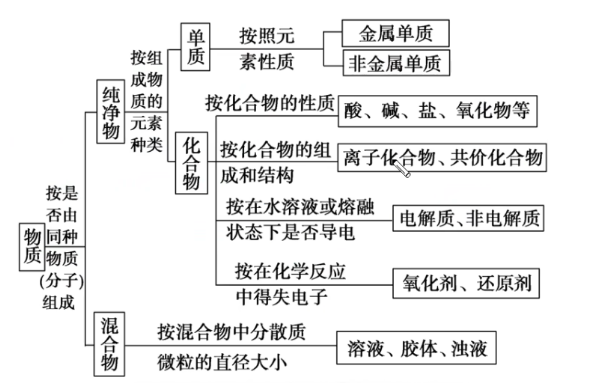
\includegraphics[width=0.75\linewidth]{Classification.png}
    \caption{Classification of substances}
    \label{fig_classification}
    \end{figure}
    
\CUPTWOCOL 
%%% END OF FIRST PAGE IN LARGE-LAYOUT NEEDS TO BE MARKED. This commands does nothing in medium and small layouts. %%%

\subsection{氧化物}
    \begin{itemize}
        \item 定义:氧元素与另外一种化学元素组成的二元化合物 
    \end{itemize}

    \begin{figure}[hbt!]
        \centering
        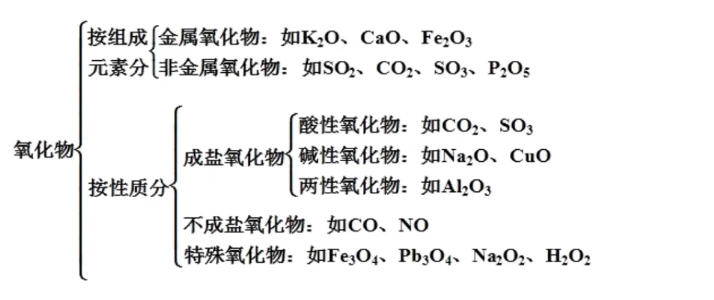
\includegraphics[width=0.75\linewidth]{oxide.png}
        \caption{oxide}
        \label{fig_oxide}
        \end{figure}
    \noindent\schemestart
        \chemfig{Fe_3O_4\+8HCl=2FeCl_3\+FeCl_2\+4H_2O}
    \schemestop
    \\
        \ce{Pb3O4 + 4HNO3 -> PbO2 + 2Pb(NO3)2 + 2H2O}\\
        \noindent \textsf{注:}碱性氧化物一定是金属氧化物

\subsubsection{Insert C head here}
Subsubsection text here. Lorem ipsum dolor sit amet, consectetur adipiscing elit, sed do eiusmod tempor incididunt ut labore et dolore magna aliqua. Lorem ipsum dolor sit amet, consectetur adipiscing elit, sed do eiusmod tempor incididunt ut labore et dolore magna aliqua. Lorem ipsum dolor sit amet, consectetur adipiscing elit, sed do eiusmod tempor incididunt ut labore et dolore magna aliqua. Lorem ipsum dolor sit amet, consectetur adipiscing elit, sed do eiusmod tempor incididunt ut labore et dolore magna aliqua. Lorem ipsum dolor sit amet, consectetur adipiscing elit, sed do eiusmod tempor incididunt ut labore et dolore magna aliqua. 

Lorem ipsum dolor sit amet, consectetur adipiscing elit, sed do eiusmod tempor incididunt ut labore et dolore magna aliqua. Lorem ipsum dolor sit amet, consectetur adipiscing elit, sed do\endnote{A footnote/endnote} eiusmod tempor incididunt ut labore et dolore magna aliqua. 

\section{Equations}

Sample equations. Lorem ipsum dolor sit amet, consectetur adipiscing elit, sed do eiusmod tempor incididunt ut labore et dolore magna aliqua. Lorem ipsum dolor sit amet, consectetur\endnote{Another footnote/endnote} adipiscing elit, sed do eiusmod tempor incididunt ut labore et dolore magna aliqua. Lorem ipsum dolor sit amet, consectetur adipiscing elit, sed do eiusmod tempor incididunt ut labore et dolore magna aliqua. Lorem ipsum dolor sit amet, consectetur adipiscing elit, sed do eiusmod tempor incididunt ut labore et dolore magna aliqua. Lorem ipsum dolor sit amet, consectetur adipiscing elit, sed do eiusmod tempor incididunt ut labore et dolore magna aliqua. 


%%% Numbered equation
\begin{equation}
\begin{aligned}\label{eq:first}
\frac{\partial u(t,x)}{\partial t} = Au(t,x) \left(1-\frac{u(t,x)}{K}\right)
 -B\frac{u(t-\tau,x) w(t,x)}{1+Eu(t-\tau,x)},\\
\frac{\partial w(t,x)}{\partial t} =\delta \frac{\partial^2w(t,x)}{\partial x^2}-Cw(t,x)
+D\frac{u(t-\tau,x)w(t,x)}{1+Eu(t-\tau,x)},
\end{aligned}
\end{equation}

Lorem ipsum dolor sit amet, consectetur adipiscing elit, sed do eiusmod tempor incididunt ut labore et dolore magna aliqua. Lorem ipsum dolor sit amet, consectetur adipiscing elit, sed do eiusmod tempor incididunt ut labore et dolore magna aliqua. Lorem ipsum dolor sit amet, consectetur adipiscing elit, sed do eiusmod tempor incididunt ut labore et dolore magna aliqua. 

\begin{align}\label{eq:another}
\begin{split}
\frac{dU}{dt} &=\alpha U(t)(\gamma -U(t))-\frac{U(t-\tau)W(t)}{1+U(t-\tau)},\\
\frac{dW}{dt} &=-W(t)+\beta\frac{U(t-\tau)W(t)}{1+U(t-\tau)}.
\end{split}
\end{align}


%%%% Unnumbered equation
\begin{align*}
&\frac{\partial(F_1,F_2)}{\partial(c,\omega)}_{(c_0,\omega_0)} = \left|
\begin{array}{ll}
\frac{\partial F_1}{\partial c} &\frac{\partial F_1}{\partial \omega} \\\noalign{\vskip3pt}
\frac{\partial F_2}{\partial c}&\frac{\partial F_2}{\partial \omega}
\end{array}\right|_{(c_0,\omega_0)}\\
&\quad=-4c_0q\omega_0 -4c_0\omega_0p^2 =-4c_0\omega_0(q+p^2)>0.
\end{align*}


\section{Figures \& Tables}

The output for a single-column figure is in Figure~\ref{fig_sim}.  Lorem ipsum dolor sit amet, consectetur adipiscing elit, sed do eiusmod tempor incididunt ut labore et dolore magna aliqua. Lorem ipsum dolor sit amet, consectetur adipiscing elit, sed do eiusmod tempor incididunt ut labore et dolore magna aliqua. Lorem ipsum dolor sit amet, consectetur adipiscing elit, sed do eiusmod tempor incididunt ut labore et dolore magna aliqua. 

Lorem ipsum dolor sit amet, consectetur adipiscing elit, sed do eiusmod tempor incididunt ut labore et dolore magna aliqua. Lorem ipsum dolor sit amet, consectetur adipiscing elit, sed do eiusmod tempor incididunt ut labore et dolore magna aliqua. Lorem ipsum dolor sit amet, consectetur adipiscing elit, sed do eiusmod tempor incididunt ut labore et dolore magna aliqua. 

%See Figure~\ref{fig_wide} for a double-column figure; this is always at the top of a following page.


\begin{figure}[hbt!]
\centering
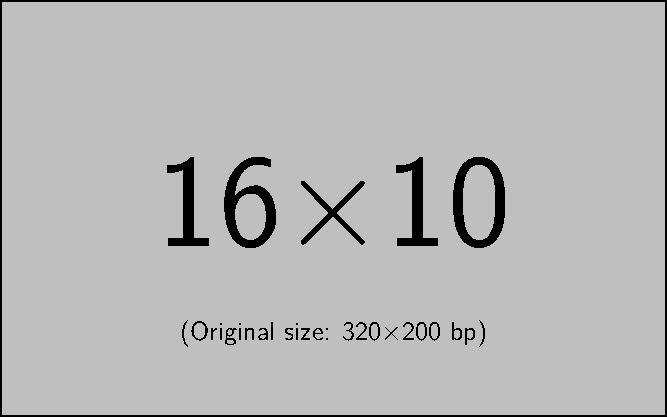
\includegraphics[width=0.75\linewidth]{example-image-16x10.pdf}
\caption{Insert figure caption here}
\label{fig_sim}
\end{figure}


\begin{figure*}
\centering
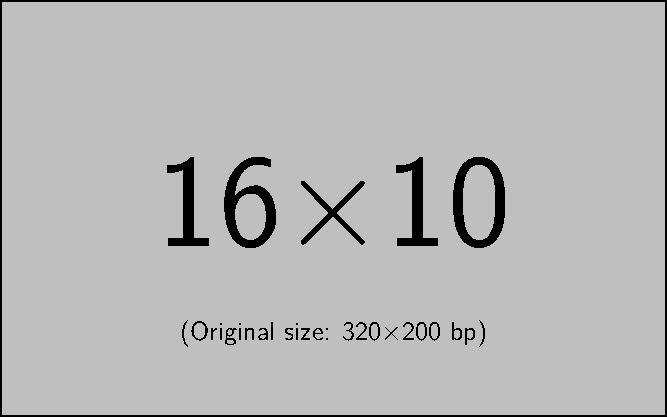
\includegraphics[width=0.8\linewidth]{example-image-16x10.pdf}
\caption{Insert figure caption here}
\label{fig_wide}
\end{figure*}


See example table in Table~\ref{table_example}.

\begin{table}[hbt!]
\begin{threeparttable}
\caption{An Example of a Table}
\label{table_example}
\begin{tabular}{llll}
\toprule
\headrow Column head 1 & Column head 2  & Column head 3 & Column head 4\\
\midrule
One\tnote{a} & Two&three three &four\\ 
\midrule
Three & Four&three three\tnote{b} &four\\
\bottomrule
\end{tabular}
\begin{tablenotes}[hang]
\item[]Table note
\item[a]First note
\item[b]Another table note
\end{tablenotes}
\end{threeparttable}
\end{table}


\section{Conclusion}
The conclusion text goes here.


\begin{acknowledgement}
Insert the Acknowledgment text here.
\end{acknowledgement}

\paragraph{Funding Statement}

This research was supported by grants from the <funder-name> <doi> (<award ID>); <funder-name> <doi> (<award ID>).

\paragraph{Competing Interests}

A statement about any financial, professional, contractual or personal relationships or situations that could be perceived to impact the presentation of the work --- or `None' if none exist.

\paragraph{Data Availability Statement}

A statement about how to access data, code and other materials allowing users to understand, verify and replicate findings --- e.g. Replication data and code can be found in Harvard Dataverse: \verb+\url{https://doi.org/link}+.



%\endnote in some journals will behave like \footnote; and \printendnotes will not output anything. 
\printendnotes

\printbibliography

\appendix

\section{Example Appendix Section}

Lorem ipsum dolor sit amet, consectetur adipiscing elit, sed do eiusmod tempor incididunt ut labore et dolore magna aliqua. Lorem ipsum dolor sit amet, consectetur adipiscing elit, sed do eiusmod tempor incididunt ut labore et dolore magna aliqua. Lorem ipsum dolor sit amet, consectetur adipiscing elit, sed do eiusmod tempor incididunt ut labore et dolore magna aliqua. 


\end{document}
